\def\extl(#1, #2){\fill (#1, #2) circle (0.05); \fill[opacity = 0.3, blue] (#1, #2) circle (0.1);  } %external vertex to the left (x,y)
\def\extr(#1, #2){\fill (#1, #2) circle (0.05); \fill[opacity = 0.3, green!50!black] (#1, #2) circle (0.1);  } %external vertex to the right (x,y)

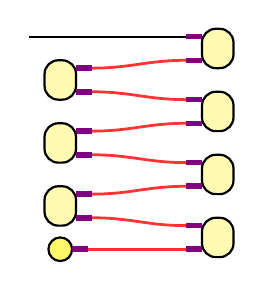
\begin{tikzpicture}
%vertices a^*, a, B
\filldraw[fill = yellow!60!white, thick] (-1,0.1) circle (0.15);

\filldraw[thick, rounded corners = 5, fill = yellow!30!white] (0.8,0) rectangle ++(0.4,0.5);
\filldraw[thick, rounded corners = 5, fill = yellow!30!white] (-1.2,0.4) rectangle ++(0.4,0.5);
\filldraw[thick, rounded corners = 5, fill = yellow!30!white] (0.8,0.8) rectangle ++(0.4,0.5);
\filldraw[thick, rounded corners = 5, fill = yellow!30!white] (-1.2,1.2) rectangle ++(0.4,0.5);
\filldraw[thick, rounded corners = 5, fill = yellow!30!white] (0.8,1.6) rectangle ++(0.4,0.5);
\filldraw[thick, rounded corners = 5, fill = yellow!30!white] (-1.2,2) rectangle ++(0.4,0.5);
\filldraw[thick, rounded corners = 5, fill = yellow!30!white] (0.8,2.4) rectangle ++(0.4,0.5);

%connectors
\draw[line width = 2, red!50!blue] (-0.85,0.1) -- ++(0.2,0);
\draw[line width = 2, red!50!blue] (0.8,0.1) -- ++(-0.2,0);
\draw[line width = 2, red!50!blue] (0.8,0.4) -- ++(-0.2,0);
\draw[line width = 2, red!50!blue] (-0.8,0.5) -- ++(0.2,0);
\draw[line width = 2, red!50!blue] (-0.8,0.8) -- ++(0.2,0);
\draw[line width = 2, red!50!blue] (0.8,0.9) -- ++(-0.2,0);
\draw[line width = 2, red!50!blue] (0.8,1.2) -- ++(-0.2,0);
\draw[line width = 2, red!50!blue] (-0.8,1.3) -- ++(0.2,0);
\draw[line width = 2, red!50!blue] (-0.8,1.6) -- ++(0.2,0);
\draw[line width = 2, red!50!blue] (0.8,1.7) -- ++(-0.2,0);
\draw[line width = 2, red!50!blue] (0.8,2) -- ++(-0.2,0);
\draw[line width = 2, red!50!blue] (-0.8,2.1) -- ++(0.2,0);
\draw[line width = 2, red!50!blue] (-0.8,2.4) -- ++(0.2,0);
\draw[line width = 2, red!50!blue] (0.8,2.5) -- ++(-0.2,0);
\draw[line width = 2, red!50!blue] (0.8,2.8) -- ++(-0.2,0);

%contractions
\draw[red, opacity = .8, line width = 1] (-0.65,0.1) -- ++(1.25,0);
\draw[red, opacity = .8, line width = 1] (-0.6,0.5) .. controls ++(0.5,0) and ++(-0.5,0) .. (0.6,0.4);
\draw[red, opacity = .8, line width = 1] (-0.6,0.8) .. controls ++(0.5,0) and ++(-0.5,0) .. (0.6,0.9);
\draw[red, opacity = .8, line width = 1] (-0.6,1.3) .. controls ++(0.5,0) and ++(-0.5,0) .. (0.6,1.2);
\draw[red, opacity = .8, line width = 1] (-0.6,1.6) .. controls ++(0.5,0) and ++(-0.5,0) .. (0.6,1.7);
\draw[red, opacity = .8, line width = 1] (-0.6,2.1) .. controls ++(0.5,0) and ++(-0.5,0) .. (0.6,2);
\draw[red, opacity = .8, line width = 1] (-0.6,2.4) .. controls ++(0.5,0) and ++(-0.5,0) .. (0.6,2.5);

%leg
\draw[thick] (0.6,2.8) -- (-1.4,2.8); \extl(-1.4, 2.8)


\end{tikzpicture}